\chapter{Team assignments}

In this chapter, we are describing motivation, development, support and usage of team assignments. This functionality was developped in summer of 2015 and then used and tested on Modern Approaches to Webdesign course during winter semester of 2016 at our faculty. Since then, multiple courses used team assignment functionality in Courses 2 Learning management system.

\section{Motivation}

Computer Science students are often taught many different types of algorithms, matematics and programmings languages. This is very beneficial to them since many hard skills will be reqired in their future career. But on the other side of this, these students are lackings skills in teamwork, constructive critisism, the ability of self\-reflection or job evaluation.  These skills are essential in ther future jobs or science career however none or very little effort is put to teach students these skills. 


This is why, throughout this work, we are introducing new concepts of assignments for students. These concepts are focused to teach students how to work in teams, teach them constructive critisism or self\-reflection. In this chapter, we describe implementing and usage of one of these concepts, team assignments. With this term, we mean an assignment, which students solve in small teams, which is beneficial for them in multiple ways. This way, student can pick any part of the project he wants to solve. What is more, we reqire peer and team reviews, which can give him feedback on how well he did it. 

This work is also a subject of many other researchers at our faculty such as Veronika Dropcova's research \cite{dropcova}, which is focusing on how students interact with each other and solve this assignments. In this work we focus mostly on implementation and support for this research.


\section{Specifications and semantics}
Now, let's describe in detail specifications and semantics of team assignments in Courses 2 learning management system. This description was is a result of long process, which we brainstormed and developed throughout whole winter semester of 2016. We will describe in detail, how teacher can create, edit and manage a team assignment, and what actions are expected out of students.

\section{Team assignment creation}
The teacher can create a team assignment in teacher's assignment interface. This interface is the same as for creating a normal assignment. The only difference is that teacher must allow the assignment to be team assignment, set deadlines for team forming and fill, how many students he expects to be in each team. The teacher can set lowest and highest number of students in each group without any limitations.

\subsection{Team forming}
After the start time of team forming has passed and before team forming deadlines, students are required to create or join a team. This is implemented as shown on figure \ref{team_forming}. Leader of the team can enter team name, which has to be unique for the course. After he created the team, he automatically joins this team and is reqired to invite his classmates to join. There is a limitation of how many students can be invited, based on maximum number of students in one team. This means that he can only invite as many friends as is the maximum number allowed by the teacher. He can, however, delete this invites and invite a different classmate. Also, any member of the team can invite another student of the course.

\begin{figure}[h]
    \centering
    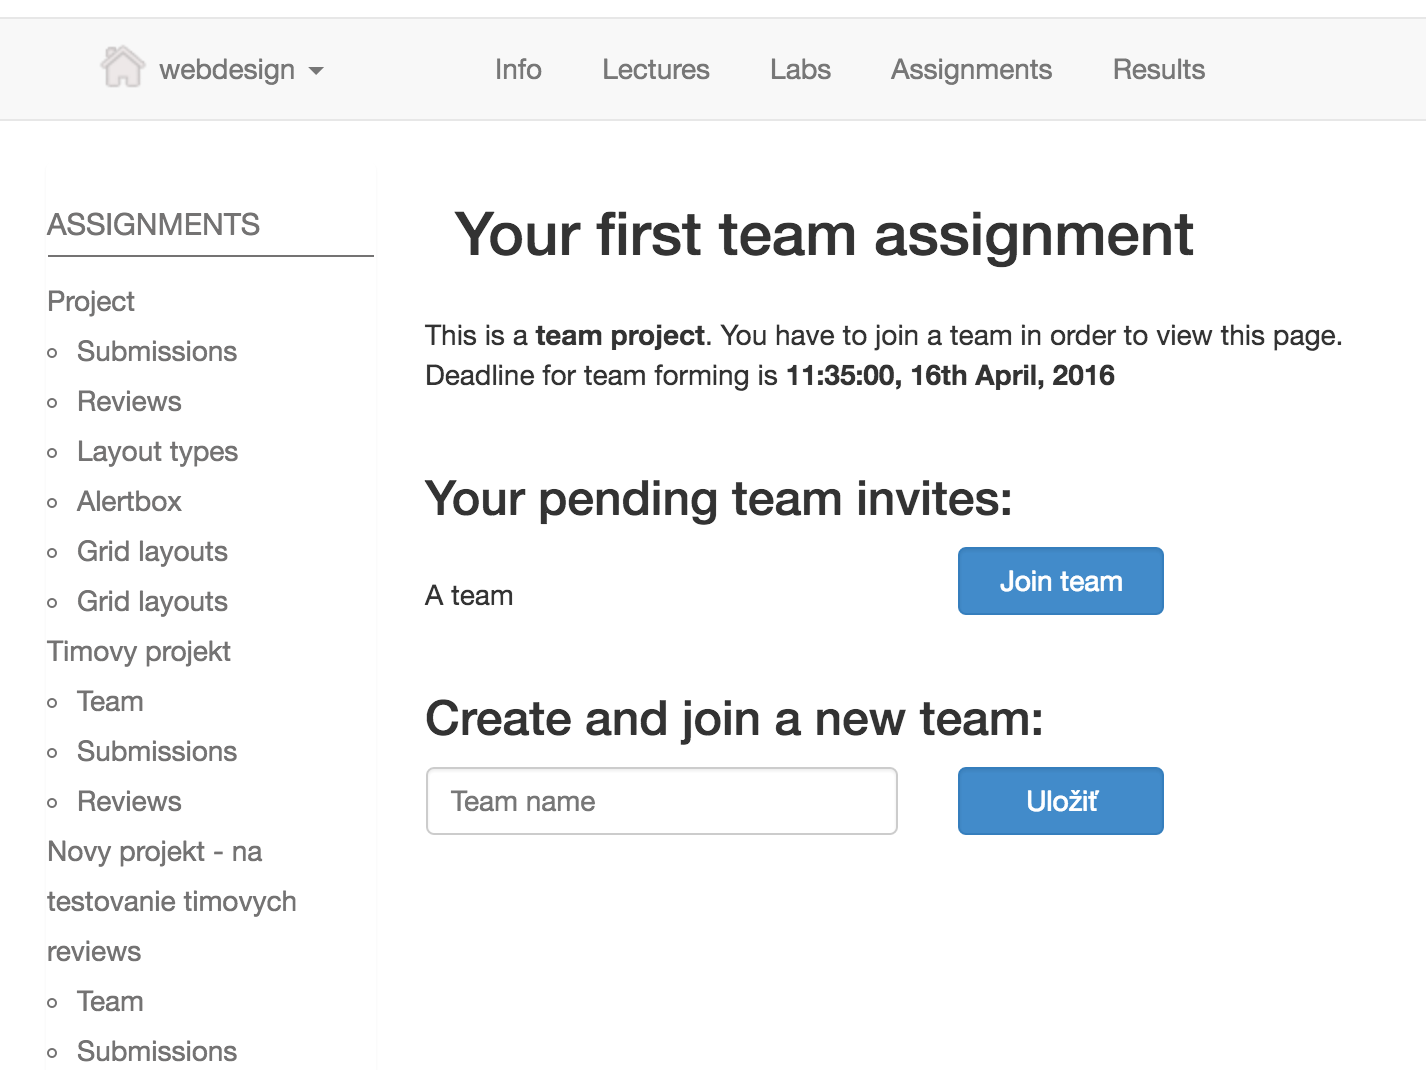
\includegraphics[width=\textwidth]{images/teamforming.png}
    \caption{Team forming}
    \label{team_forming}
\end{figure}

If the student accepts an invite, all his other invites are made invalid so these teams can invite different students. This student can also leave the team if he wants, but the team has to invite him again if they want him to join again. There is also no option to kick another team member from team, he can only leave willingly. If all members of the team left, the team is deleted and dismissed.

Another thing to mention, while the team does not have enough members specified by the teacher, there is a notification shown to each member. This is done to ensure that the team does not forget about this.

After the team forming deadline, no student can join, create nor leave the team. After this deadline, only teacher can edit team members and still create new team. 

The teacher can in administration see the list of the teams as shown on figure \ref{team_forming}. During the development, we tried multiple types of interfaces and this is the one that was selected. This interface offers simple access to each student and team forming or editing.

After the team forming period, the teacher must check if all of the students joined a team and if not, assign them into a team. He must also check whether all of the teams have enough members. As seen on figure \ref{team_forming}, the table is a list of students and their teams. The table is sorted and groupped by team name to offer easy navigation. Then the table is sorted by student name. The last results are students which do not have any team. Their names are highlighted by a slight blue collor. With green color are marked teams that does not have enough members. And, if by any chance, team managed to have more members than is allowed by teacher (the teacher could lesser this value so the existing full teams would not met the maximum count of team members condition) these are marked red. So, basically, for any colored line, the teacher must take an action.


\begin{figure}[h]
    \centering
    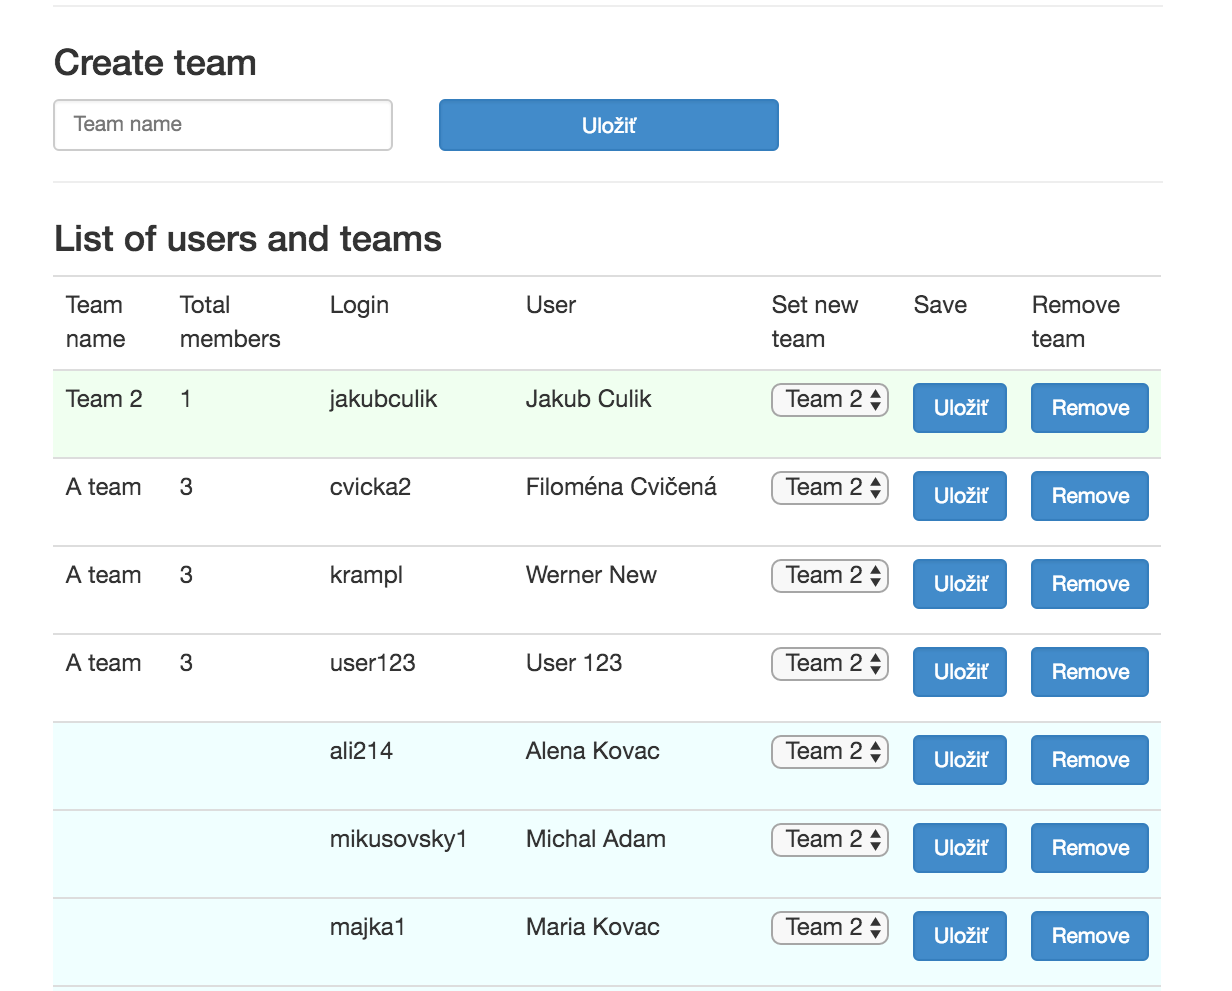
\includegraphics[width=\textwidth]{images/teamadmin.png}
    \caption{Team administration}
    \label{team_forming}
\end{figure}


\subsection{Assignment submission}

\subsection{Peer review}

\subsection{Teamwork review}

\subsection{Teacher's evaluation}

\section{Implementation}
odofjasdofij